\documentclass[12pt,a4paper,utf8x]{article}
%\usepackage [frenchb]{babel}
\usepackage [english]{babel}

% Pour pouvoir dessiner des graphes
\usepackage{tikz}
\usepackage{tikz,fullpage}
\usetikzlibrary{arrows,%
                petri,%
                topaths}%
\usepackage{tkz-berge}
\usepackage[position=top]{subfig}

%Maths
%\usepackage{fc}
\usepackage[mathcal]{euscript}
%\usepackage{eufrak}
\usepackage{amsfonts}


% Pour pouvoir utiliser 
\usepackage{ucs}
\usepackage[utf8x]{inputenc}
\usepackage{hyperref}


\usepackage{url} % Pour avoir de belles url
\usepackage {geometry}
%\usepackage[printonlyused,withpage]{acronym}


% Pour mettre du code source
\usepackage {listings}
% Pour pouvoir passer en pa
\usepackage{lscape}

%\usepackage{color}

% Pour pouvr faire plusieurs colonnes
\usepackage {multicol}
% POur crééer un index
\usepackage{makeidx}
%Pour les images
\usepackage{graphicx}
\makeindex

% Pour les entetes de page
% \usepackage{fancyheadings}
%\pagestyle{fancy}
%\renewcommand{\sectionmark}[1]{\markboth{#1}{}} 
%\renewcommand{\subsectionmark}[1]{\markright{#1}} 

% Pour l'interligne de 1.5
\usepackage {setspace}
% Pour les marges de la page
\geometry{a4paper, top=2.5cm, bottom=3.5cm, left=1.5cm, right=1.5cm, marginparwidth=1.2cm}

\parskip=5pt %% distance entre § (paragraphe)
\sloppy %% respecter toujours la marge de droite 

% Pour les pénalités :
\interfootnotelinepenalty=150 %note de bas de page
\widowpenalty=150 %% veuves et orphelines
\clubpenalty=150 

%Pour la longueur de l'indentation des paragraphes
\setlength{\parindent}{15mm}



%%%% debut macro pour enlever le nom chapitre %%%%
\makeatletter
\def\@makechapterhead#1{%
  \vspace*{50\p@}%
  {\parindent \z@ \raggedright \normalfont
    \interlinepenalty\@M
    \ifnum \c@secnumdepth >\m@ne
        \Huge\bfseries \thechapter\quad
    \fi
    \Huge \bfseries #1\par\nobreak
    \vskip 40\p@
  }}

\def\@makeschapterhead#1{%
  \vspace*{50\p@}%
  {\parindent \z@ \raggedright
    \normalfont
    \interlinepenalty\@M
    \Huge \bfseries  #1\par\nobreak
    \vskip 40\p@
  }}
\makeatother
%%%% fin macro %%%%

%Couverture 

\title
{
	\normalsize{Javascript viewer\\
	For NMR and MS experiment\\
	}
	\vspace{15mm}
	\textbf{\Huge{Tutorial to know how it works}}
}
\author{Samy Deghou\\
  Elève ingénieur 5ème année\\
  Majeure Bioinformatique\\
	\vspace{45mm}
}

\date{	
	\normalsize{\textbf{E}uropean \textbf{B}ioinformatics \textbf{I}nstitute\\
          Chemoinformatics and  Metabolism team\\
          \textbf{Metabolight Project}\\
          Sponsored by...\\ \textbf{Mark Rijnbeek}
	\vspace{5mm}
	}
}

\begin{document}

\maketitle
\clearpage


\tableofcontents
\clearpage

% Pour avoir un interligne de 1,5
\begin{onehalfspace}

\section{Introduction}
\subsection{What does it do?}
The aim is to build a viewer displaying the output of a chemical experiment:

-Mass Spectra experiment

-NMR experiment\\
Each output experiment provides the information about:

-The molecule studied.

-Its spectra.

-The additional information about the condition of the experiment\\
Hence, the viewer must \textbf{displays} the\textbf{ molecule} along with its \textbf{spectrum}. Besides, we want it to be \textbf{interactive} with the user, e.g when the user mouse over one peak, it has to \textbf{highlights} and highlights the corresponding atoms it is linked to(in the case of a \href{http://en.wikipedia.org/wiki/Nuclear\_magnetic\_resonance}{NMR experiment}) and it has to display the corresponding fragment(s) (in case of a \href{http://en.wikipedia.org/wiki/Mass\_spectrometry}{MS experiment}).
\subsection{How do we do it?}
The entire viewer is build with JavaScript and use the \href{http://code.google.com/closure/}{google closure library}

\subsubsection{Google Closure}

In summary, the Closure Library is a JavaScript library which is based on a modulable architecture. It provides cross-browser functions for DOM manipulations and events, AJAX and JSON, as well as more high-level objects such as User Interface widgets and controls.
For instance and in our case, it provides the tools to design a canvas editor, and all the objects to have a control over this canvas.
\clearpage


\section{The entry point}

Our Input data is a file in a \textbf{cml file}, which is a standart of xml. The file contains the information generated by the output of the experiment. It holds either MS data, or NMR data.\\
    \begin{figure}[h]
    \begin{centering}
    \caption{Example of cml file}
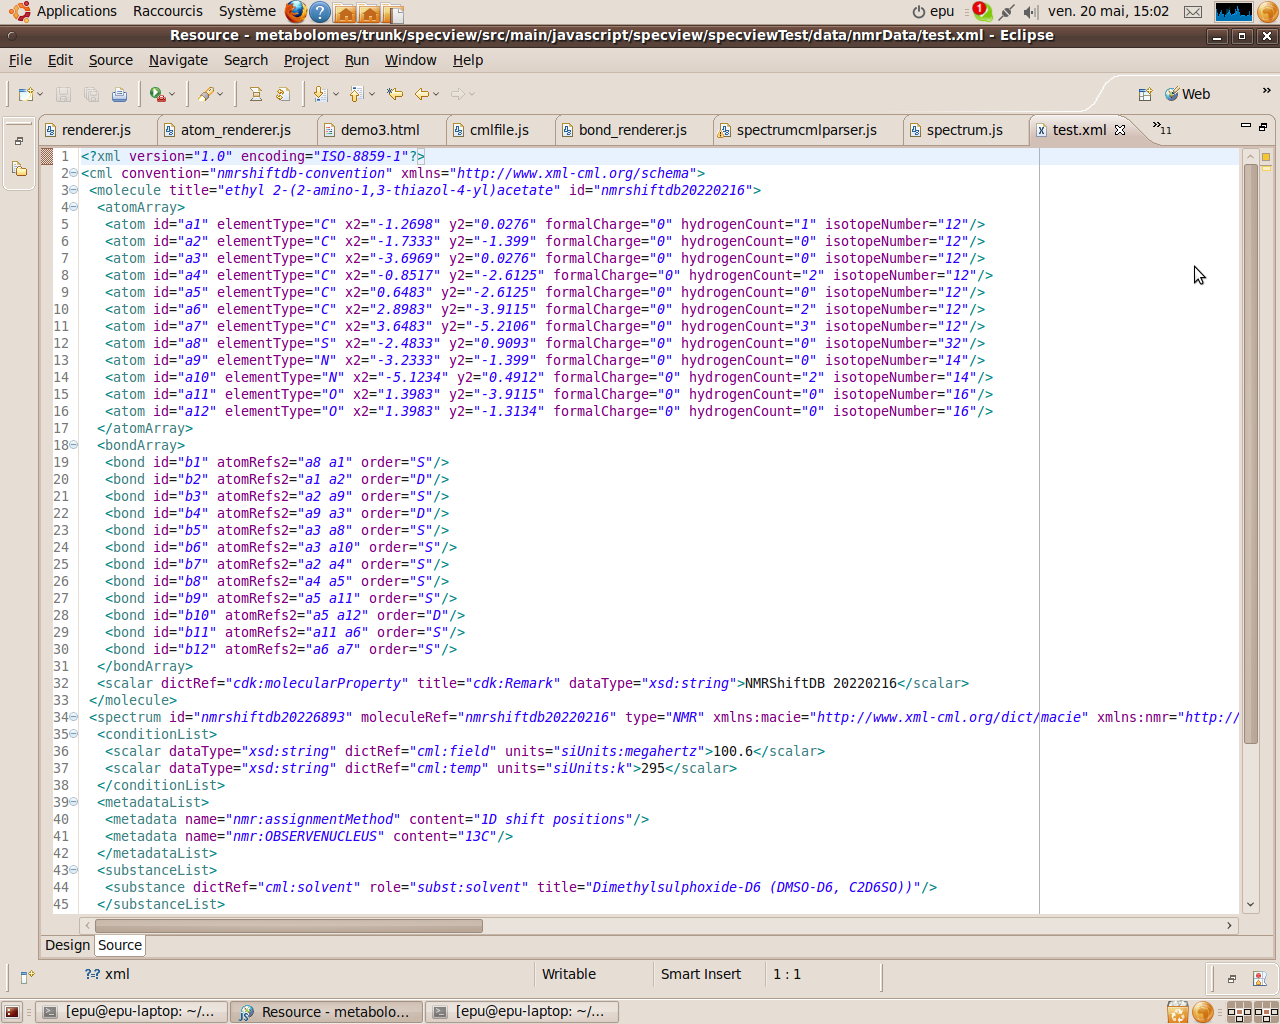
\includegraphics[width=190mm,height=160mm]{./images/sampleCML}
%    \label{subd}
    \end{centering}
    \end{figure}

\subsection{What does it contain?}

This file provides all the information required in order to build a \textbf{molecule} and a \textbf{spectrum}.
THe molecule consists in a liste of \textbf{\textit{atoms}}:
    \begin{figure}[h]
    \begin{centering}
    \caption{A list of atoms}
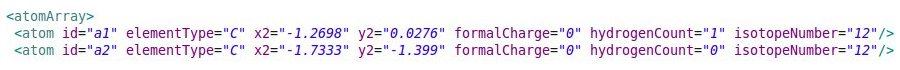
\includegraphics[width=180mm,height=13mm]{./images/atoms}
   \end{centering}
The list of atoms contains all the informations to identify the entities of the molecules. The important point is that the coordinates it contains are relative coordinates. In order to display the atoms on the screen, they have to be transformed into actual coordinates, ``pixel coordinates''.
    \end{figure}
    \begin{figure}[h]
    \begin{centering}
    \caption{A list of bonds}
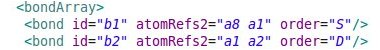
\includegraphics[width=75mm,height=7mm]{./images/bonds}
    \end{centering}
    \end{figure}
The bonds refer to 2 atoms by their id. It is possible, that single order bond have a certain stereo specificity. In that case, the bond $``b_i''$ would have a tag $``bondStereo''$ specifying the orientation of the bond.
    \begin{figure}[h]
    \begin{centering}
    \caption{Example of peak annotation for a NMR experiment}
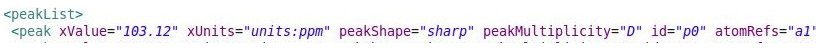
\includegraphics[width=150mm,height=10mm]{./images/annotation}
    \end{centering}
    \end{figure}
Thie information about the \textbf{peak} os probably the most important. This where the \textbf{annotation} stands. Each peak has a \textbf{\href{http://www.w3schools.com/schema/el\_field.asp}{field}} or a \textbf{\href{http://www.w3schools.com/dom/dom\_node.asp}{child}} that refer to:\\

-One or multiple \textbf{atom} if the file holds \textbf{NMR} experiment

-One or multiple \textbf{molecule} if the file holds \textbf{MS} experiment\\
The objects are mentioned by their inner identifier(identifier found in the file, e.g $a_1$,$a_2$... for an atom and $m_1$,$m_2$... for a molecule).

Furthermore, MS files can have fields tagged ``scalar information'' at the end of each molecule. These file holds additional information on the moleculem, such as physico chemical properties, inChi key, other identifiers...\\
Finally, the file contains other information regarding the experiment within the tag ``condition'' and ``metadata''.



\clearpage


\section{Create a JavaScript Object}
Now, in order to display the content of the file, we decide to create an object, called $``metaSpecObject''$. This object is a generic object that can contains all the data to represent a molecule along with its spectrum and the information to allow the cross talk between the two entities.
    \begin{figure}[h]
    \begin{centering}
    \caption{Attributes of the metaSpecObject}
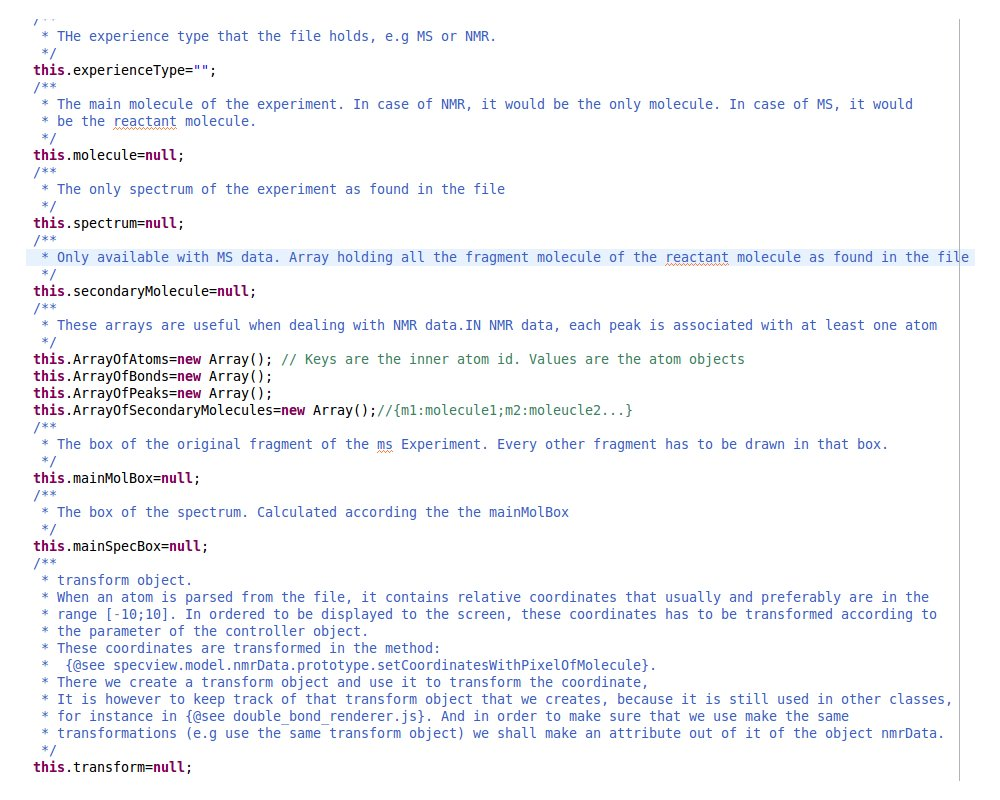
\includegraphics[width=195mm,height=150mm]{./images/metaSpecObjectAttributes}
%    \label{subd}
    \end{centering}
    \end{figure}
\clearpage

The aim is to conceive an object that holds all the elements to create a molecule object, a spectrum object, and keeping track of the relation between one peak and another object(either a molecule or an atom).
This is way, each peak is considered as being an object (@see peak.js) and has several fields that may relate to its corresponding objects:\\

    \begin{figure}[h]
    \begin{centering}
    \caption{The object Peak}
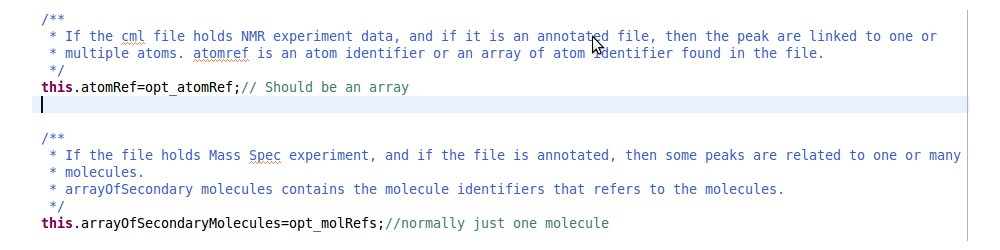
\includegraphics[width=195mm,height=50mm]{./images/peakAnnotation}
%    \label{subd}
    \end{centering}
    \end{figure}
With these two fields, whenever a peak is linked to another object,  it is possible to track this object.




\clearpage


\section{The parser}

So far the parser takes cml files (version 2008-->2010) and works with Firefox and Internet Explorer.\\
N.B: Javascript does not conveniently work with file input stream, so the most convenient way to deal with it is to:

(i)   Make a string out of the cml file.

(ii)  Load the cml string into an XML object.

(iii) Parse the object and extract the information we want to create the metaSpecObject

\subsection{A few points}
Before rendering everything, some things have to be done
\subsubsection{SetCoordinatesWithPixel}
The file contains relative coordinates, that is, they need to be transfomed into actual coordinates in order to be properly rendered.
This is done in the method setCoordinateWithPixel:
    \begin{figure}[h]
    \begin{centering}
    \caption{The object Peak}
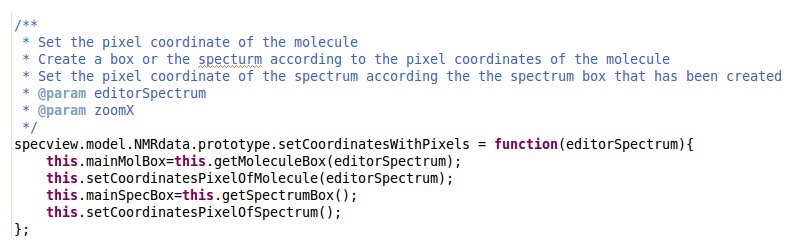
\includegraphics[width=195mm,height=55mm]{./images/setCoordinatesWithPixel}
%    \label{subd}
    \end{centering}
    \end{figure}
That method is an instance method of the metaSpecObject. The first step is to define:

(i) Get the molecule box where the molecule will be drawn.

(ii) Set the pixel coordinates of the molecule.

(iii) Set the spectrum box according to the molecule box.

(iv) Set the pixel coordinates of the spectrum(e.g of all the peaks)
\\

\textbf{Get the molecule box}

    \begin{figure}[h]
    \begin{centering}
    \caption{Get the molecule box}
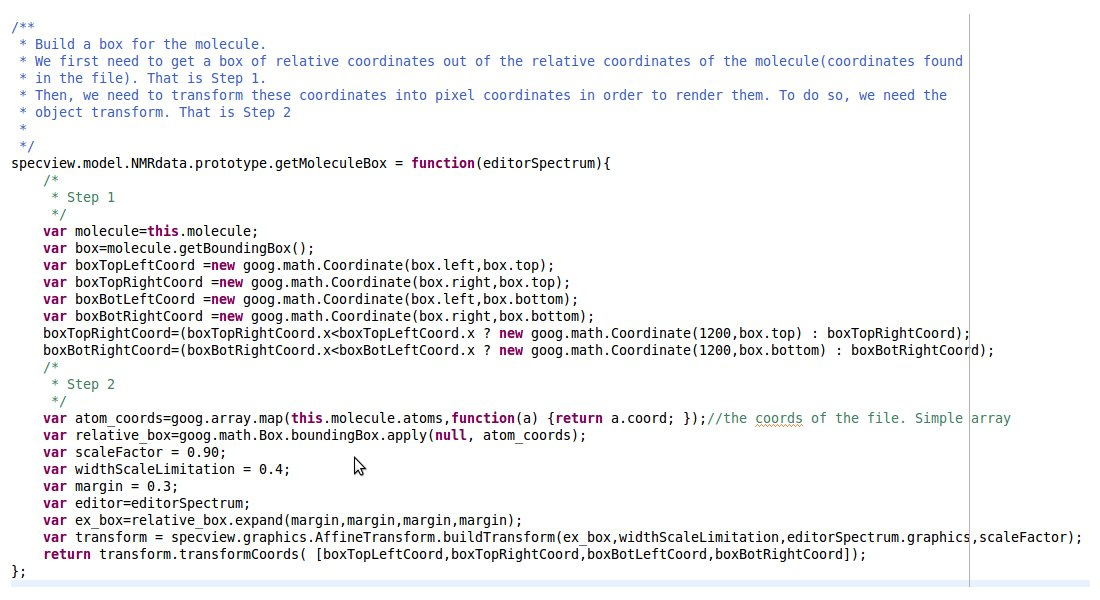
\includegraphics[width=195mm,height=100mm]{./images/getMoleculeBox}
%    \label{subd}
    \end{centering}
    \end{figure}

The method take as an input the editor object, and return an array of 4 coordinates (pixel coordinates) that will be used to draw the molecule box.

\textbf{Transform object}

In order to transform relative coordinates into actual coordinates, we need to take into account the dimension(e.g width andheight) of the canvas editor (which is an attribute of the editor object). This is the reason why the method has an input ``editorSpectrum'' which is the editor object. This is used in the method to create a ``transform'' object which does the transformation from realtive coordinates into actual coordinates.
\clearpage
\textbf{Set the molecule coordinates}

    \begin{figure}[h]
    \begin{centering}
    \caption{Set the molecule Coordinates}
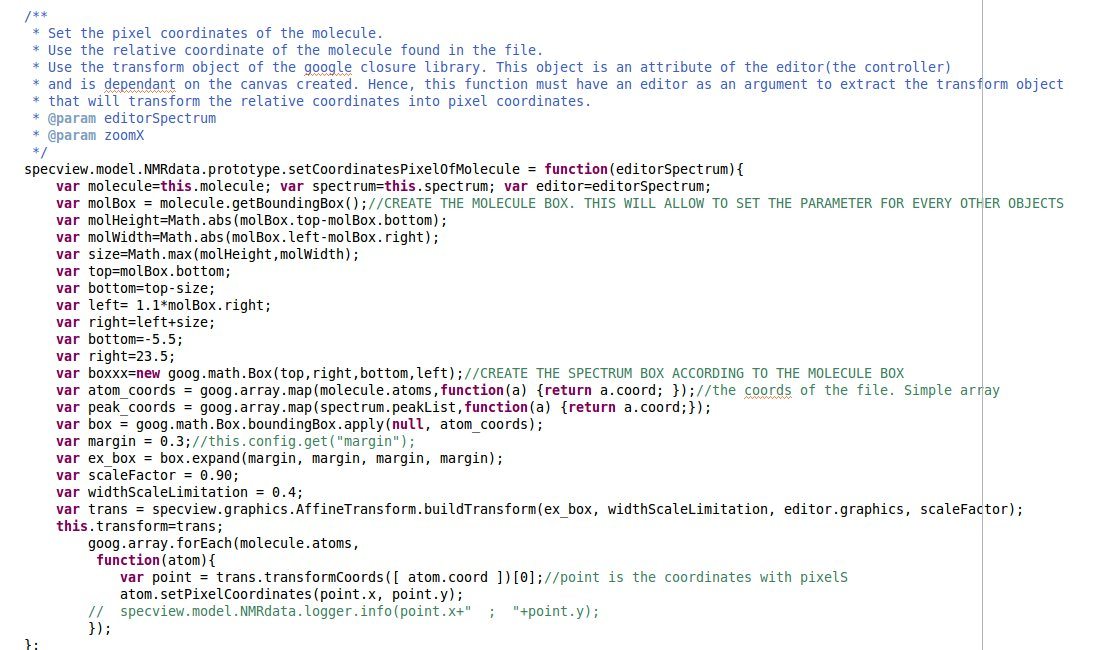
\includegraphics[width=195mm,height=120mm]{./images/setMoleculeCoordinates}
%    \label{subd}
    \end{centering}
    \end{figure}
\clearpage
\textbf{Get the spectrum box}
    \begin{figure}[h]
    \begin{centering}
    \caption{Get the spectrum box}
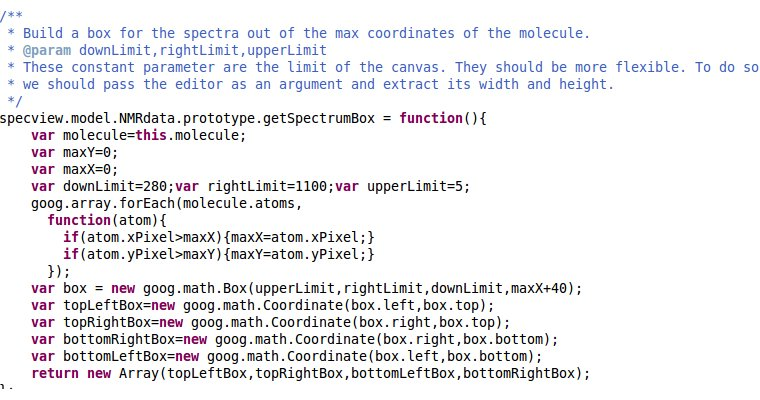
\includegraphics[width=155mm,height=68mm]{./images/getSpecBox}
%    \label{subd}
    \end{centering}
    \end{figure}
\textbf{Set the spectrum pixel coordinates}
    \begin{figure}[h]
    \begin{centering}
    \caption{Set the pixel coordinates pixel}
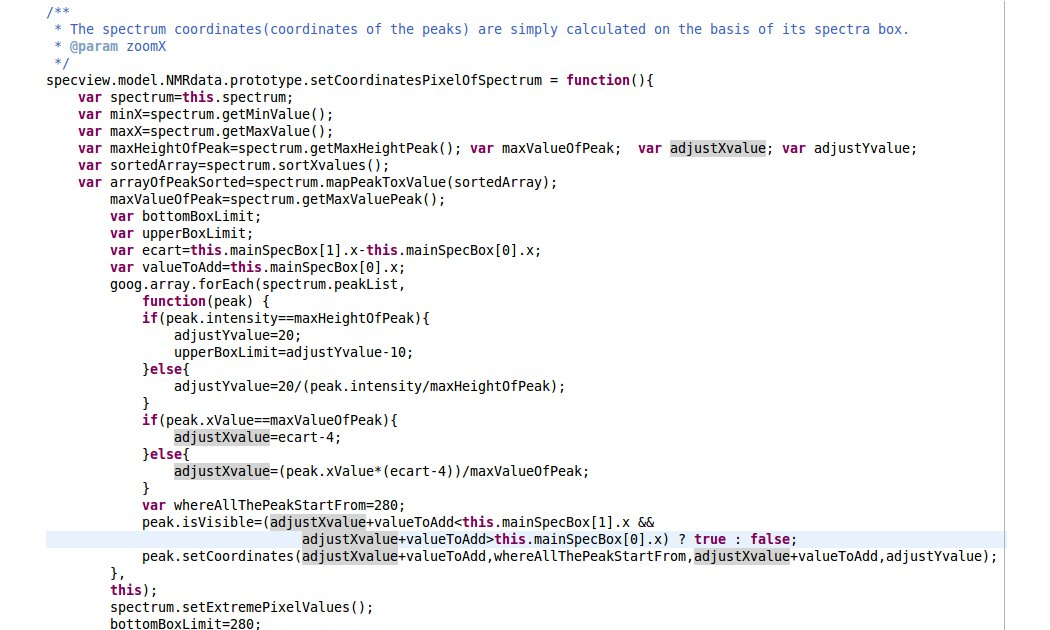
\includegraphics[width=180mm,height=80mm]{./images/setSpecPixel}
%    \label{subd}
    \end{centering}
    \end{figure}

\subsubsection{Mapping}
The viewer has to be interactive. When the user mouse over peaks or atom or bonds, it has to highlights all the objects in relation with the focused object. To do so, we have to create a ``neighborlist'' object.\\

\textbf{The ``neighborlist'' object}

The controller object contains one attribute ``neighborlist''. It is a class for locating the objects nearest to a specified coordinate. That way, when the mouse will hover an object, the controller will know that at this precise coordinate is located an object that has to be highlighted.\\
When we create a ``neighborlist'' object, we create an associative array whose keys are coordinates and value are the object at the given coordinate.
\clearpage


\section{How to display everything?}

Right after the ``neighborlist'' object has been created, we can render the whole thing.
    \begin{figure}[h]
    \begin{centering}
    \caption{THe instance method ``render'' of the controller object}
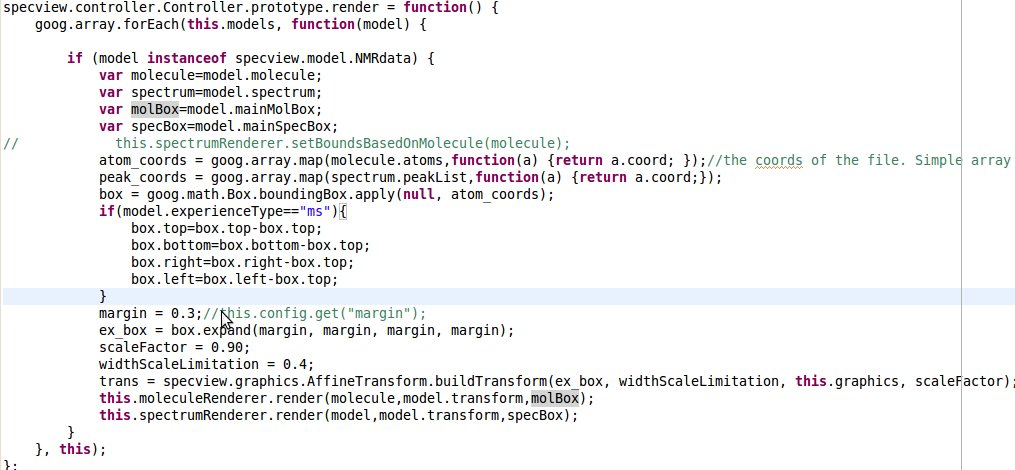
\includegraphics[width=200mm,height=95mm]{./images/renderController}
%    \label{subd}
    \end{centering}
    \end{figure}

At the end of this method are called             this.\textbf{moleculeRenderer}.render(molecule,model.transform,molBox) and 
            this.\textbf{spectrumRenderer}.render(model,model.transform,specBox).
``molceuleRenderer'' and ``spectrumRenderer'' are attributes of the controller object. More precisely they are classes  to render molecule and spectrum objects on graphics objects. These classes contain a instance method named ``render'' which properly draw the molecule(respectibely spectrum) object on the graphics object.
\clearpage

\textbf{Example of a renderer class}

    \begin{figure}[h]
    \begin{centering}
    \caption{The instance method render of the class spectrumRenderer}
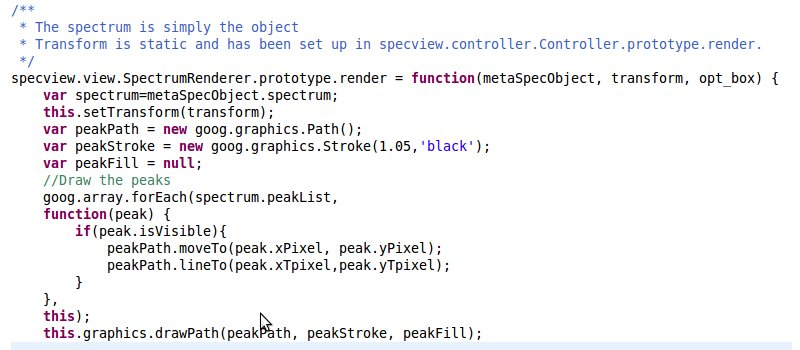
\includegraphics[width=190mm,height=75mm]{./images/spectrumRenderer}
%    \label{subd}
    \end{centering}
    \end{figure}

At each ``\textbf{this.graphics.drawPath(peakPath, peakStroke, peakFill)}'' a new peak is drawn on the canvas editor. 
\clearpage


\section{Simple workflow}
    \begin{figure}[h]
    \begin{centering}
    \caption{Step to render the experiment}
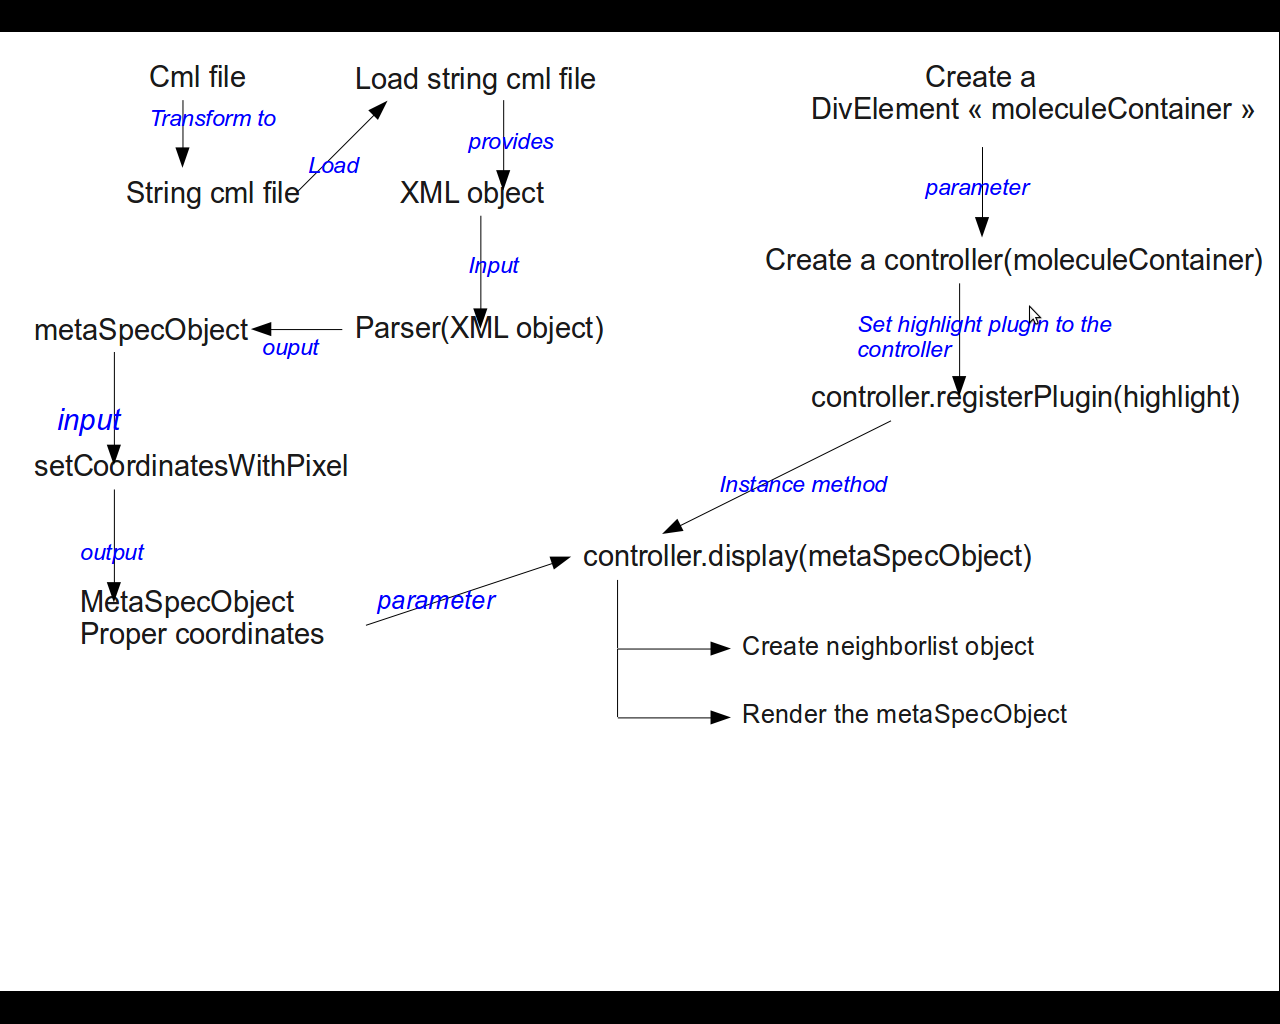
\includegraphics[width=190mm,height=150mm]{./images/workflow1}
%    \label{subd}
    \end{centering}
    \end{figure}
\clearpage


\section{Highlight}

The highlight process is a plugin that can be registered into the controller object.



\input{specificities}

%\input{Conclusion}

% Pour finir l'interligne de 1,5
\end{onehalfspace}

%----------------------------------------
% Pour la bibliographie
%----------------------------------------
% Citer tous les ouvrages/références
\nocite{*}
% Trier par ordre d'apparition
%bibliographystyle{unsrt}
% Pour le sty1e de la biblio
\bibliographystyle{unsrt}



\printindex

\appendix


\end{document}
